\section{Field}
The Field consists of several components; the Track, Pickup and Launch zones, three Obstacles, the Target and the Sprint. A general description of each component follows below. Models and dimensioned drawings of each of the Field’s components can be found in the {\href{https://mercury.okstate.edu/content/mercury-challenge}{2019 Track Pack}}.

\begin{figure}[H]
	\centering
	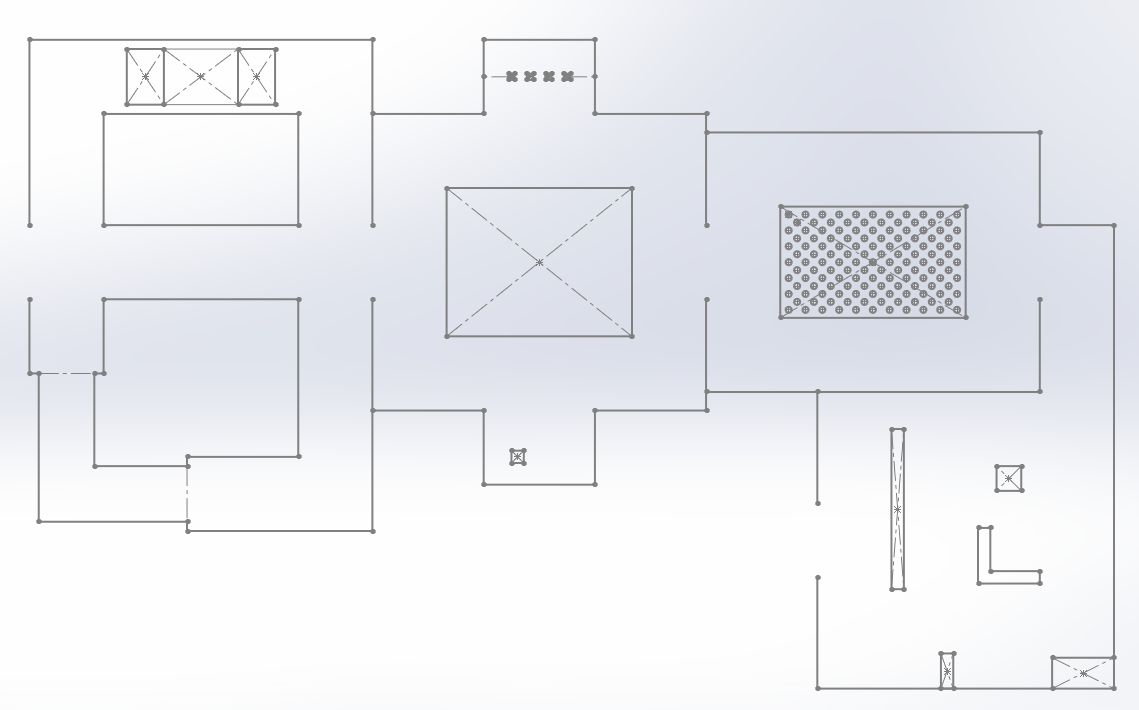
\includegraphics[width=.85\textwidth]{images/track_overview_wlabels.png}
	\caption{Field Overview}
	\label{fig:field} 
\end{figure}

\subsection{Track}
The Track is defined as a 24 inch wide path that is bounded on either side by 3 inch high walls. The walls used at the Competition will be constructed from foam board of the type that is easily obtainable from craft stores; 1/8 inch thick with a matte, white paper surface. The track floor will be terazzo.

\subsection{Bypasses}
The 2020 Competition Track does include paths that bypass most Obstacles. Teams may choose to bypass any or all of the Obstacles during a run. See section \ref{bypass} for details.

\subsection{Rough Terrain}
The Rough Terrain section is a 3 feet wide by 5 feet long area covered with an array of domes aligned in a diagonal grid pattern. The domes are 3D printed plastic with a base diameter of 2 inches and a height of 1/2 inch. There will be walls on the long edges of the section, with bypass paths extending another 24 inches beyond the section walls. This Obstacles tests the durability and agility of the robot.

\subsection{Tunnel}
The Tunnel is an L-shaped wooden structure with openings on either end that are 12 inches high by 18 inches wide. The interior is dark. This Obstacle tests the maneuverability of the robot in a confined space with limited visibility.

\subsection{Bridge}
The Bridge is 24 inches wide with a smooth wooden surface and no guard walls. The climb is 30 degrees with 12 inch rise, followed by a 24 inch span and a 30 degree descent. This Obstacle tests the robot’s ability to move in a controlled manner on an inclined surface.

\subsection{Object Identification and Handling}
	\subsubsection{Pick-up zone}
		There are four objects in the pick-up zone. Each of them contains an elctromagnetic coil and will be generat

\subsection{Obstacle Avoidance}
The Obstacle Avoidance section is defined as a 6 feet wide by 8 feet long rectangular area. The Robot must navigate from the start to the finish without contacting walls or obstacles. Obstacles will be 2 inches deep by 4 inches high and of varied length. They will be \textbf{bright orange}. There will be at least one path with a minimum of 24 inches between obstacles. This section will be offered in 3 versions of varying autonomy.

\begin{itemize}
    \item Manual - Known Placement
    
        The Network will remain enabled and the Operator will have full control of the Robot as it navigates the section. If this option is chosen, the section will be laid out as defined below.
    \item Autonomous - Known Placement
    
        The Network will be disabled and the Operator will lose contact with the Robot. The Robot must be able to navigate the section autonomously. If this option is chosen, the section will be laid out as defined below.
    \item Autonomous - Unknown Placement
    
        The Network will be disabled and the Operator will lose contact with the Robot. The Robot must be able to navigate the section autonomously. If this option is chosen, the layout of obstacles in the section will be unknown to Teams until after the deadline to submit Robots on the day of the Competition. 
        
\end{itemize}